

\section{Natureza jurídica}\label{s:natur}

\begin{multicols}{2}

A natureza jurídica, ou tipo societário, é um meio de determinar a estrutura e funcionamento de uma empresa. De acordo com o \href{http://www.snis.gov.br/downloads/manuais-atualizados/drenagem/Natureza_Juridica.pdf}{Glossário do SNIS} a natureza jurídica dos prestadores de serviços de saneamento podem ser: administração privada e administração pública. A administração pública pode ser direta e indireta. Destaca-se que a administração pública indireta subdivide-se em autarquia, empresa pública e sociedade de economia mista. A estrutura societária de cada uma pode ser vista no Quadro abaixo.

\end{multicols}

\vspace{1cm}

%---------------------------------------------------------------------------

\begin{myexampleblock}{Quadro 1: Natureza jurídica dos prestadores de serviços de saneamento no estado de São Paulo}\label{qua:q1}
   \textbf{Administração Pública Direta} $\rightarrow$ Prestação de serviços
públicos diretamente pelo próprio Estado. Seja ela da União, Estados e Municípios e Distrito Federal. \\
   
  \textbf{Autarquia}  $\rightarrow$ Entidade com personalidade jurídica de direito público, criada por lei específica, com patrimônio próprio, atribuições públicas
específicas e capacidade de auto administrar-se, sob controle estadual ou municipal. \\

  \textbf{Empresa pública} $\rightarrow$ Entidade de personalidade jurídica de direito privado com patrimônio próprio e capital exclusivo da União, do Estado ou do
Município. Tem sua instituição autorizada por lei para prestação de serviço público passível de exploração econômica. \\

  \textbf{Empresa Privada} $\rightarrow$ São as empresas que não estão ligadas ao Estado. \\

  \textbf{Sociedade de economia mista} $\rightarrow$ Entidade de personalidade jurídica de direito privado com capital público e privado, maioria pública. 
\end{myexampleblock} 
%{\small Fonte: Elaborado pelos autores.}

%---------------------------------------------------------------------------

\vspace{1cm}

\begin{multicols}{2}
 A maior parte dos municípios paulistas tem como natureza jurídica dos prestadores de serviços de água e esgoto a sociedade de economia mista, como pode ser visto na Tabela \ref{tab:prop}. Destaca-se que esses dados são de 2019. Dos 375 munícipios cuja natureza jurídica é mista, 371 são atendidos pela Companhia de Saneamento Básico do Estado de São Paulo (SABESP) que é uma Sociedade Anônima de economia mista que atende 28,8 milhões de pessoas com abastecimento de água e 24,9 milhões com serviços de esgoto\footnote{Essas informações podem ser vistas no \href{http://site.sabesp.com.br/site/interna/Default.aspx?secaoId=505}{site da SABESP}. }. Os demais municípios são atendidos pelo Serviço Autônomo de Água e Esgoto (SAAE) ou pelas suas respectivas prefeituras. 

\end{multicols}



\begin{table}[H]\centering 
\begin{minipage}{0.8\textwidth}
  \caption{Natureza jurídica dos prestadores de serviços de abastecimento de água e esgoto dos municípios paulistas - 2019} 
  \label{tab:prop} 
\begin{tabular}{@{\extracolsep{5pt}} ccc} 
\\[-1.8ex]\hline 
\hline \\[-1.8ex] 
Natureza Jurídica & Número de municípios & Proporção de municípios \\ 
\hline \\[-1.8ex] 
	Adm. pública direta 	& $145$ 	& $22,48\%$ \\ 
	Autarquia 			& $88$ 	& $13,64\%$ \\ 
	Empresa privada 		& $23$ 	& $3,57\%$ \\ 
	Empresa pública 		& $2$ 	& $0,3\%$ \\ 
	Mista 				& $375$ & $58,14\%$ \\ 
    Sem Classificação	& $12$  & $1,86\%$ \\ 
\hline \\[-1.8ex] 
	Total               & 645    & $100\%$ \\
\hline \\[-1.8ex] 
\end{tabular} 
	\footnotesize \\
	Fonte: Elaborado pelos autores com dados do SNIS.
\end{minipage}
\end{table} 






\begin{multicols}{2}
	Na Figura \ref{f:maps15}	 apresentamos a distribuição espacial dos prestadores de serviços de água e esgoto nos municípios paulistas. Nota-se que nas regiões de Sorocaba, Itapeva, Registro, Grande São Paulo, Santos, São José dos Campos, Presidente Prudente e São José do Rio Preto são onde predominam a sociedade de economia mista\footnote{Detalhes sobre a localização das regiões administrativas de São Paulo podem ser vistos no Apêndice \ref{ap1}.}. 
	
\end{multicols}


\begin{figure}[H]
        \centering
        	\begin{minipage}{0.6\textwidth}	
                \caption{Distribuição espacial dos prestadores de serviços de água e esgoto nos municípios paulistas}
                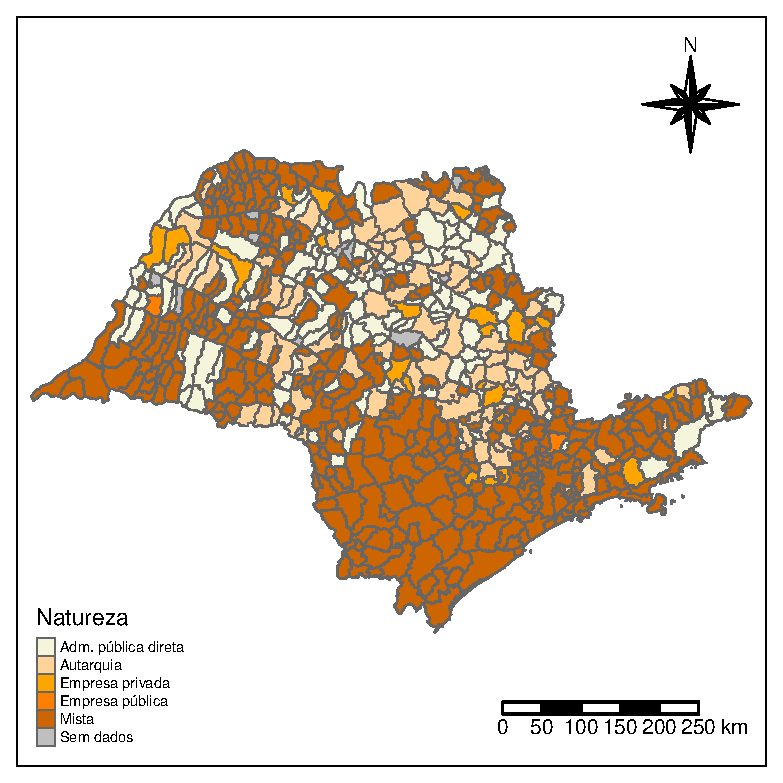
\includegraphics[scale=0.8]{figures/m1.eps}                 
            	\footnotesize \\
            		Fonte: Elaborado pelos autores com dados do SNIS.
    	\label{f:maps15}
	\end{minipage}
\end{figure}


